\documentclass{tufte-handout}
\usepackage{amsmath}
\usepackage[utf8]{inputenc}
\usepackage{mathpazo}
\usepackage{booktabs}
\usepackage{microtype}

\usepackage{tikz}

\pagestyle{empty}


\title{Spanning USA Report}
\author{by Group Z\\ Lucas Beck, Eva Bertels, Kristin Kaltenh\"{a}user, Sune T\o nder}

\begin{document}
  \maketitle

  \section{Results}

  The following table summarizes our results:
  
  \bigskip\noindent
  \begin{tabular}{lr}
    \toprule
    Input file & MST total weight \\ \midrule
    USA-highway-miles.txt	 & 16598 \\
    tinyEWG-alpha.txt & 181 \\ \bottomrule
  \end{tabular}

  \bigskip
\noindent The MST we found in tinyEWG-alpha.txt can be drawn like this:

  \medskip
  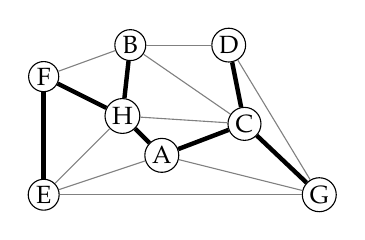
\begin{tikzpicture}[
      scale = .5,
      every node/.style = {
        circle, draw, black, inner sep = 1pt, font = \small},
      every path/.style = {gray}
      ]
    \node (A) at (3,1) {A}; % 0
    \node (B) at (2.2,3.8) {B}; % 1
    \node (C) at (5.1,1.8) {C}; % 2
    \node (D) at (4.7,3.8) {D}; % 3
    \node (E) at (0,0) {E}; % 4
    \node (F) at (0,3) {F}; % 5
    \node (G) at (7,0) {G}; % 6
    \node (H) at (2,2) {H}; % 7
    \draw (E)--(F);
    \draw (E)--(H);
    \draw (F)--(H);
    \draw (A)--(H);
    \draw (B)--(F);
    \draw (A)--(E);
    \draw (C)--(D);
    \draw (B)--(H);
    \draw (A)--(C);
    \draw (B)--(C);
    \draw (B)--(D);
    \draw (C)--(H);
    \draw (G)--(C);
    \draw (D)--(G);
    \draw (G)--(A);
    \draw (G)--(E);
    \begin{scope}[every path/.style={ultra thick}]
      \draw(B)--(H);
      \draw(A)--(C);
      \draw(C)--(D);
      \draw(E)--(F);
      \draw(F)--(H);
      \draw(G)--(C);
      \draw(A)--(H);
    \end{scope}
  \end{tikzpicture}


  \section{Implementation details}

We implemented the algorithm of Prim, using \texttt{PrimMST.java} from \textit{Sedgewick and Wayne}.
  The edges are created by passing the integers we associated with the vertices using a \texttt{HashMap}, as well as the weight as a double.

\bigskip

Prim's algorithm runs in $O(m\log n)$. 
  Adding edges to the weighted graph takes linear time in edges (\textit{m}), which leads to a total running time of $O(m + m \log n)$.

  %Use $n$ for the number of vertices, $m$ for the number of edges in the input graph.

\end{document}
